\documentclass{standalone}
% preamble: usepackage, etc.
\usepackage{tikz}
\usepackage{amsmath}

\begin{document}

\chapter{路径规划问题}
在这一章,我们引入路径规划问题,给出其严格的数学定义。然后介绍随着现实交通网络的复杂化,路径规划问题所出现的新的形式和挑战,并给出其数学形式。通过这一章,我们将详细阐述我们的工作所解决的问题,这将有利于在随后的相关章节中强化学习算法的设计和实验。
\section{路径规划问题的数学形式}
路径规划问题,如绪论1.2节所述,根据问题建模形式,其算法分为基于图的搜索算法和基于采样的规划方法。在本文中,我们使用基于图的搜索算法,然后给出其相应的数学形式。\par
令 $v\in \{1,2,3...n\}$表示图中的某个顶点,假设有$n$个顶点。令$e_{i,j}$表示图中的一条从点$i$到点$j$的一条边,假设共有$m$条边。令$V$ 表示图中节点的集合,令$E=\{e_{i,j})| i,j \in V \}$表示图中边的集合。
令$f:E \to \mathbb{R}$ 表示为一个将图中的任意一条边映射到某一实数集上的函数,在静态的最短路径问题中,该函数一般等价于路径长度,但在本文中,为了使模型和算法应用于多种场景中,我们将其定义为抽象的损失函数,即通过某条边的损失,以使得定义能够适应于复杂的路径规划场景。$f$函数的输入包括但不限于某条边,在不同问题中,可能会有额外的输入信息以计算该函数值,例如在带有转弯额外惩罚的场景中,车辆是否转弯也作为函数的输入以计算损失值。则由以上定义可得一个有向图定义为$G=(V, E, f)$,其包含一个点集$V$,一个边集$E$和一个损失函数$f$。

我们定义$P=\{v_1, v_2,...,v_k\}$为图中的一条路径,路径的长度或总损失定义为$L(P) = \sum_{i=1}^{j-1} f(e_{v_i,v_{i+1}})$。基于以上定义,最短路径规划问题可以被定义为:在图$G$中,给定某一起始点$v_s$和终止点$v_t$,找到某一条路径$P_{optimal}$使得$L(P_{optimal})$最小,公式定义如下:
\begin{center}
\begin{equation}
P_{optimal}(v_s, v_t) = argmin_{P}(L(P(v_s, v_t)))
\end{equation}
\mbox{where $v_s$ is the start node of $P$, $v_t$ is the end node of $P$}
\mbox{argmin($\cdot$)is the argument of the minimum function}
\end{center}

一个简单的实例如图\ref{fig2shortest}所示,标注深色的边表示了从节点 A 到节点 F 的最短路径。
\begin{figure}[H]
    \centering
	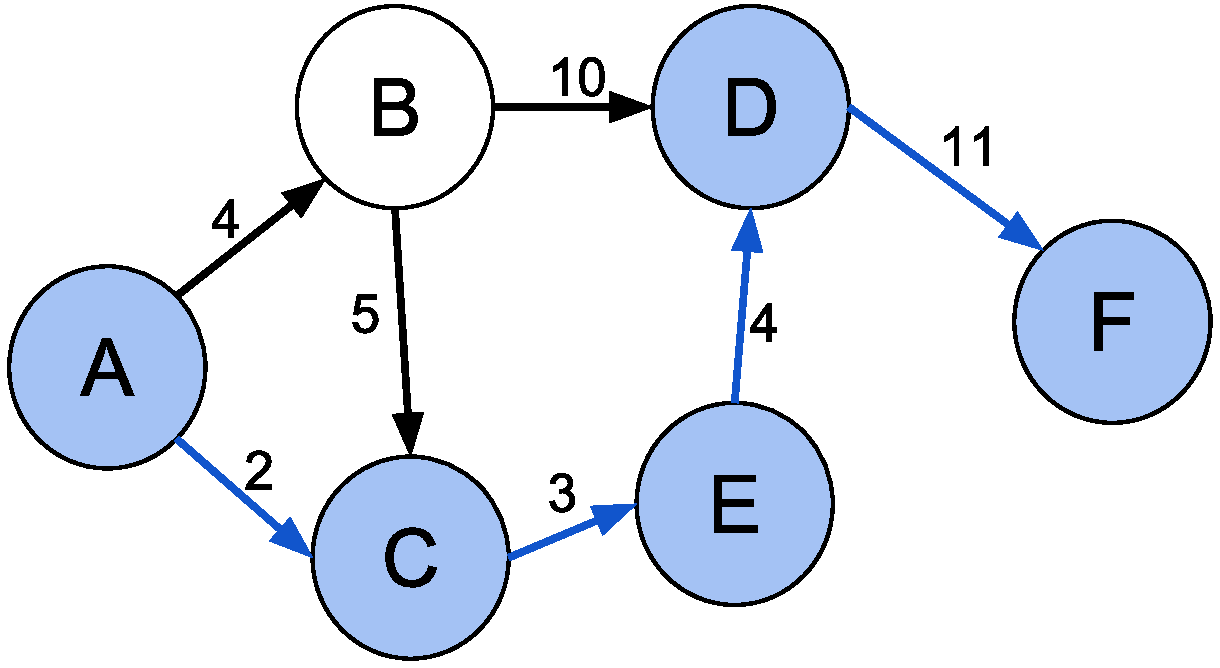
\includegraphics[width=12.0cm]{pic/2-1.pdf}
	\caption{最短路径求解示例}
	\label{fig2shortest}
\end{figure}

\section{不同场景及其数学形式}
在这一章节,我们将介绍基于2.1章节的基本最短路径问题形式的几个特殊场景,这些场景是由于随着现代交通网路的发展和复杂化,以及交通工具的扩展而出现的一些不同于传统形式的特殊场景。这些场景的出现使得我们需要对原有的问题形式进行一定的修改和重新定义,以方便我们进行相应算法的设计和实现。在本章节中将要介绍的场景也是我们将要使用强化学习进行应用和解决的场景。通过给出其数学形式上的严格定义,有助于我们在随后进行基于马尔科夫决策过程的建模和强化学习算法的设计。

\subsection{场景1:简单网格地图}
第一个场景为简单网格地图场景,设计该场景的原因在于,我们将通过这一简单的场景验证强化学习模型在路径规划问题上的可用性。在该场景中,我们通过一个二维网格表示地图,在任意一个点,在不越过地图界限的情况下,车辆可以向上下左右四个方向移动,如图\ref{figcase1}所示。令 $N$ 表示图的行数, $M$表示图的列数,左下角点的坐标为$(0,0)$,右上角的坐标为$(N-1, M-1)$。在图中,我们定义$S$ 为起点,$E$为目标点,某一时刻,车辆所处的位置由图中的$car$ 点表示。车辆在移动过程中,其每次移动距离为一个格子,边上的损失函数 定义为:
\begin{center}
    \begin{equation}
    f(e_{v_i,v_{i+1}}) = C 
\end{equation}
\mbox{$C\in\mathbb{R}$, $C\ge0$, {且$C$为常数}}
\end{center}

\begin{figure}[H]
\centering
    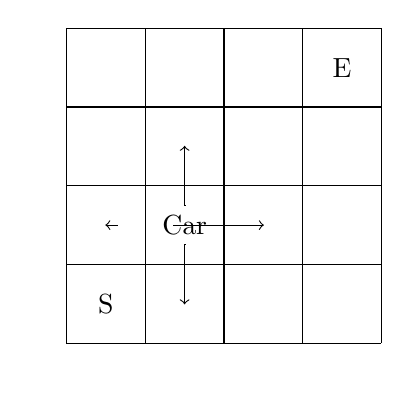
\begin{tikzpicture}[every node/.style={minimum size=1cm-\pgflinewidth, outer sep=0pt}, arrow/.style={thick}]
        \draw[step=1cm,color=black] (-2,-2) grid (2,2); 
        \node[](start) at (-1.5, -1.5) {S};
        \node[](end) at (1.5, 1.5) {E};
        \node[](car) at (-0.5, -0.5) {Car};
        
        \node[](car_up_center) at (0.0, -0.25) {};    
        \node[](car_up) at (-0.5, 1.0) {};
        
        \node[](car_down_center) at (0.0, -0.75) {};
        \node[](car_down) at (-0.5, -2.0){};
    
        \node[](car_left_center) at (-1.35, -0.5) {};
        \node[](car_left) at (-2.0, -0.5){};
    
        \node[](car_right_center) at (-0.65, -0.5) {};
        \node[](car_right) at (1.0, -0.5){};
        
        % \node[](charge site) at (-0.5, 1.5) {$t_{1}$};
        % \node[](charge site) at (1.5, -0.5) {$t_{2}$};
        \draw[->, to path={-| (\tikztotarget)}]
     	( car_up_center) edge (car_up)  (car_down_center) edge (car_down) ;
         \draw[<-, to path={-| (\tikztotarget)}]
     	(car_left) edge (car_left_center) (car_right) edge (car_right_center);
    \end{tikzpicture}
    \caption{场景1:简单网格地图}
    \label{figcase1}
\end{figure}

\subsection{场景2:带有转弯惩罚的场景}
在现实交通网络中,对最短路径计算结果具有重要影响的因素之一为转弯方向的选择,例如在图\ref{figcase1}实例中,同时存在多条从起点到终点的最短路径,但在实际交通网络中,例如中国等靠右行驶的国家中,左转往往比直行和右转具有更长的时间消耗。因此在两条最短路径行驶长度完全相同的情况下,较少左转的路径往往实际消耗的时间更少。
我们通过加入额外的转弯惩罚设计了场景2,在该场景中,在任意一条边上的移动损失函数定义为
\begin{center}
\begin{equation}
f(e_{v_i,v_{i+1}}) = \begin{cases}
C + A &\mbox{if car turn left or turn around}\\
C &\mbox{else}
\end{cases}
\end{equation}
\mbox{其中 }
$A \in\mathbb{R}, C\ge0$
\mbox{ 为常数,表示转弯的额外惩罚}
\end{center}

\subsection{场景3:带有行驶路径限制和充电桩的场景}
随着电动汽车的普及和推广,基于电动车的路径规划也作为某一特定问题被各国学者进行研究。该场景的特殊性在于,电动车普遍行驶距离较短,在进行单次路径规划中,我们在求解最短路径的同时,需要保证其在任意行驶过程中保持电量大于零,如果电量过低,需要到就近的充电桩进行充电后再行驶。
这给原始的简单网格地图的场景带来了如下变化:首先,地图中增加多个充电桩的位置,充电桩的集合被定义为 $T = \{t_{1}, t_{2}...,t_{k}\}, t_i \in V$;
同时对车辆,除去其当前位置,我们需要引入$\mathrm{power}\in[0, FULL\_POWER]$表示车辆当前剩余电量。其中 $FULL\_POWER\ge0$,表示车辆电量的最大值。修改后的地图如图\ref{figcase2}所示

\begin{figure}[H]
\centering
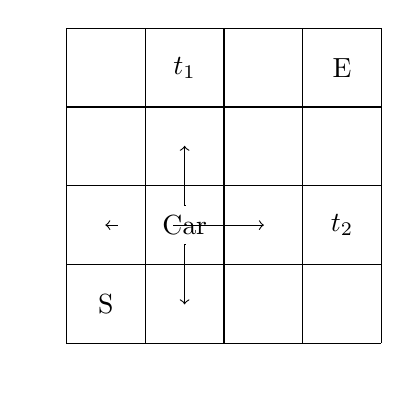
\begin{tikzpicture}[every node/.style={minimum size=1cm-\pgflinewidth, outer sep=0pt}, arrow/.style={thick}]
    \draw[step=1cm,color=black] (-2,-2) grid (2,2); 
    \node[](start) at (-1.5, -1.5) {S};
    \node[](end) at (1.5, 1.5) {E};
    \node[](car) at (-0.5, -0.5) {Car};
    
    \node[](car_up_center) at (0.0, -0.25) {};    
    \node[](car_up) at (-0.5, 1.0) {};
    
    \node[](car_down_center) at (0.0, -0.75) {};
    \node[](car_down) at (-0.5, -2.0){};

    \node[](car_left_center) at (-1.35, -0.5) {};
    \node[](car_left) at (-2.0, -0.5){};

    \node[](car_right_center) at (-0.65, -0.5) {};
    \node[](car_right) at (1.0, -0.5){};
    
    \node[](charge site) at (-0.5, 1.5) {$t_{1}$};
    \node[](charge site) at (1.5, -0.5) {$t_{2}$};
    \draw[->, to path={-| (\tikztotarget)}]
 	( car_up_center) edge (car_up)  (car_down_center) edge (car_down) ;
     \draw[<-, to path={-| (\tikztotarget)}]
 	(car_left) edge (car_left_center) (car_right) edge (car_right_center);
\end{tikzpicture}
\caption{场景3:电动车路径规划问题的网格地图}
\label{figcase2}
\end{figure}

\section{本章小结}
作为本文的正式内容的第一个章节,我们给出了路径规划问题的定义,以及出现的多个新的场景和需求。通过给出严格定义,将为下面章节我们使用强化学习解决问题提供较严格的数学形式支持。

% \subsection{场景4:动态地图环境}
% 在现实交通网络环境中,另外一个影响路径规划算法的问题为道路堵车问题,而城市道路堵车状况可以被建模为一种依赖于时间规律变化的场景。正如在1.2节提到的路径规划问题的分类,我们可以将这一问题划分到动态图或具有时序依赖的路径规划范畴中。在这个场景中,我们将基于场景1的任意一条边的行驶损耗建模成一个依赖于时间周期性变化的函数,并且使用一天作为变化的一个周期来模拟城市的堵车状态。这使得我们的路径规划算法在考虑行驶路径最短的情况下,需要考虑在不同时段下,不同路段堵车情况所带来的额外损失以求得依赖于时序的最短路径。\par
% 首先对任意一条图上的边$e_{i,j}$,我们定义重新定义场景1的函数为一个基于正太分布函数$f_{e_{i,j}}(t) = a\times N(\mu, \sigma^2) + C$,
% 表示其依赖时序变化的损耗值,我们需要针对每条边设计其参数$a, b, \mu, \sigma$的值。接下来我们将简单的构建一个典型的城市堵车状况,即在上班时段,大多车辆从城市周围进入城市中心,在下班时段,大多数车辆从城市中心向城市四周分布行驶。\par
% 因此我们首先定义城市中心位置为 $v_center$,对$v_i\in V, v_i \neq v_center$,根据二维几何空间欧氏距离的定义,其到中心的距离表示为 $D(v_center, v_i)$。我们对任意一条边$e_{i,j}$通过计算其是否使得车辆在通过它后是否远离中心分为两类$\{toWork, offWork\}$。当车在通过边$e_{i,j}$,即从点$v_i$到达$v_j$后,我们通过如下公式:
% \begin{center}
% \begin{equation}
% e_{i,j} is \begin{cases}
% toWork &\mbox{if $D(v_{center}, v_i)\leq D(v_{center}, v_j)$}\\
% offWork &\mbox{if $D(v_{center}, v_i) > D(v_{center}, v_j)$}
% \end{cases}
% \end{equation}
% \end{center}
% 现在我们按照24小时为周期,定义7-9时刻为上班高峰期,17-19为下班高峰期。通过预先定义的$v_center, \mu_{toWork}, \sigma_{toWork}, \mu_{afterWork}, \sigma_{afterWork}, a, b$,,以及用$MaxDistance$表示到中心点最远点的距离。推算出其他边的参数值。然后我们按照如下算法流程设计图计算某条边的的损耗函数的参数值。


% \begin{algorithm}[H]
%     % \DontPrintSemicolon
% 	\KwIn{G=$\{V, E\}$,\quad$v_{center}$,\quad$\mu_{toWork}$, \quad $\sigma_{toWork}$, \quad $\mu_{afterWork}$, \quad  $\sigma_{afterWork}$, \quad  $a$, \quad  $b$, \quad $MaxDistance$}
% 	\KwOut{$\sigma_{1..n}, \mu_{1..n}, a_{1..n}, b_{1..n}$}
% 	Inlization\;
% 	\Begin{
%         $\mu_{toWork} \leftarrow 8$,\;
% 	    $\sigma_{toWork} \leftarrow 1$,\;
%         $\mu_{afterWork} \leftarrow 18$,\;
%  	    $\sigma_{afterWork} \leftarrow 1$,\;
%  	    $a \leftarrow A, A > 0$,\;
%         $b \leftarrow B, B > 0$\;
% 	}
% 	\For{each edge $e_{i,j} \in E$}{
% 	    \If{$D(v_{center}, v_i)\leq D(v_{center}, v_j)$}{
% 	    $\mu_{e_{i,j}} \leftarrow \mu_{toWork} \times \frac{D(v_{center}, v_i)}{MaxDistance}$,\;
% 	    $\sigma_{e_{i,j}} \leftarrow \sigma_{toWork} \times \frac{D(v_{center}, v_i)}{MaxDistance}$,\;
% 	    }
% 	    \Else{
% 	    $\mu_{e_{i,j}} \leftarrow \mu_{offWork} \times (1 + \frac{D(v_{center}, v_i)}{MaxDistance})$,\;
% 	    $\sigma_{e_{i,j}} \leftarrow \sigma_{offWork} \times \frac{D(v_{center}, v_i)}{MaxDistance}$,\;
% 	    }
% 	}
% \caption{城市道路堵车模拟算法}
% \end{algorithm}

\end{document}